%!TEX root = ../TTK26-Summary.tex
\section{Anatomy and physiology}
Anatomy is the study of the structure of the body and its parts. Physiology is the study of the functions of the body.

\subsection{Anatomical terminology}
Tables \ref{tab:anatomical-directions} and \ref{tab:anatomical-planes} define the anatomical direction and planes of the human body, and Figures \ref{fig:directions} and \ref{fig:planes} visualize them.

\begin{table}[htbp]
  \centering
  \begin{tabularx}{\linewidth}{lX}
    \toprule
    Direction & Meaning \\
    \midrule
    anterior/ventral & front \\
    posterior/dorsal & back \\
    lateral & side \\
    proximal & near trunk or attached end of limb \\
    distal & far from trunk or attached end of limb \\
    medial & close to midline \\
    lateral & away from midline \\
    superior & higher up \\
    inferior & lower down \\
    cranial & toward the head \\
    caudal & toward the feet \\
    \bottomrule
  \end{tabularx}
  \caption{Anatomical directions}
  \label{tab:anatomical-directions}
\end{table}

\begin{figure}[htbp]
  \centering
  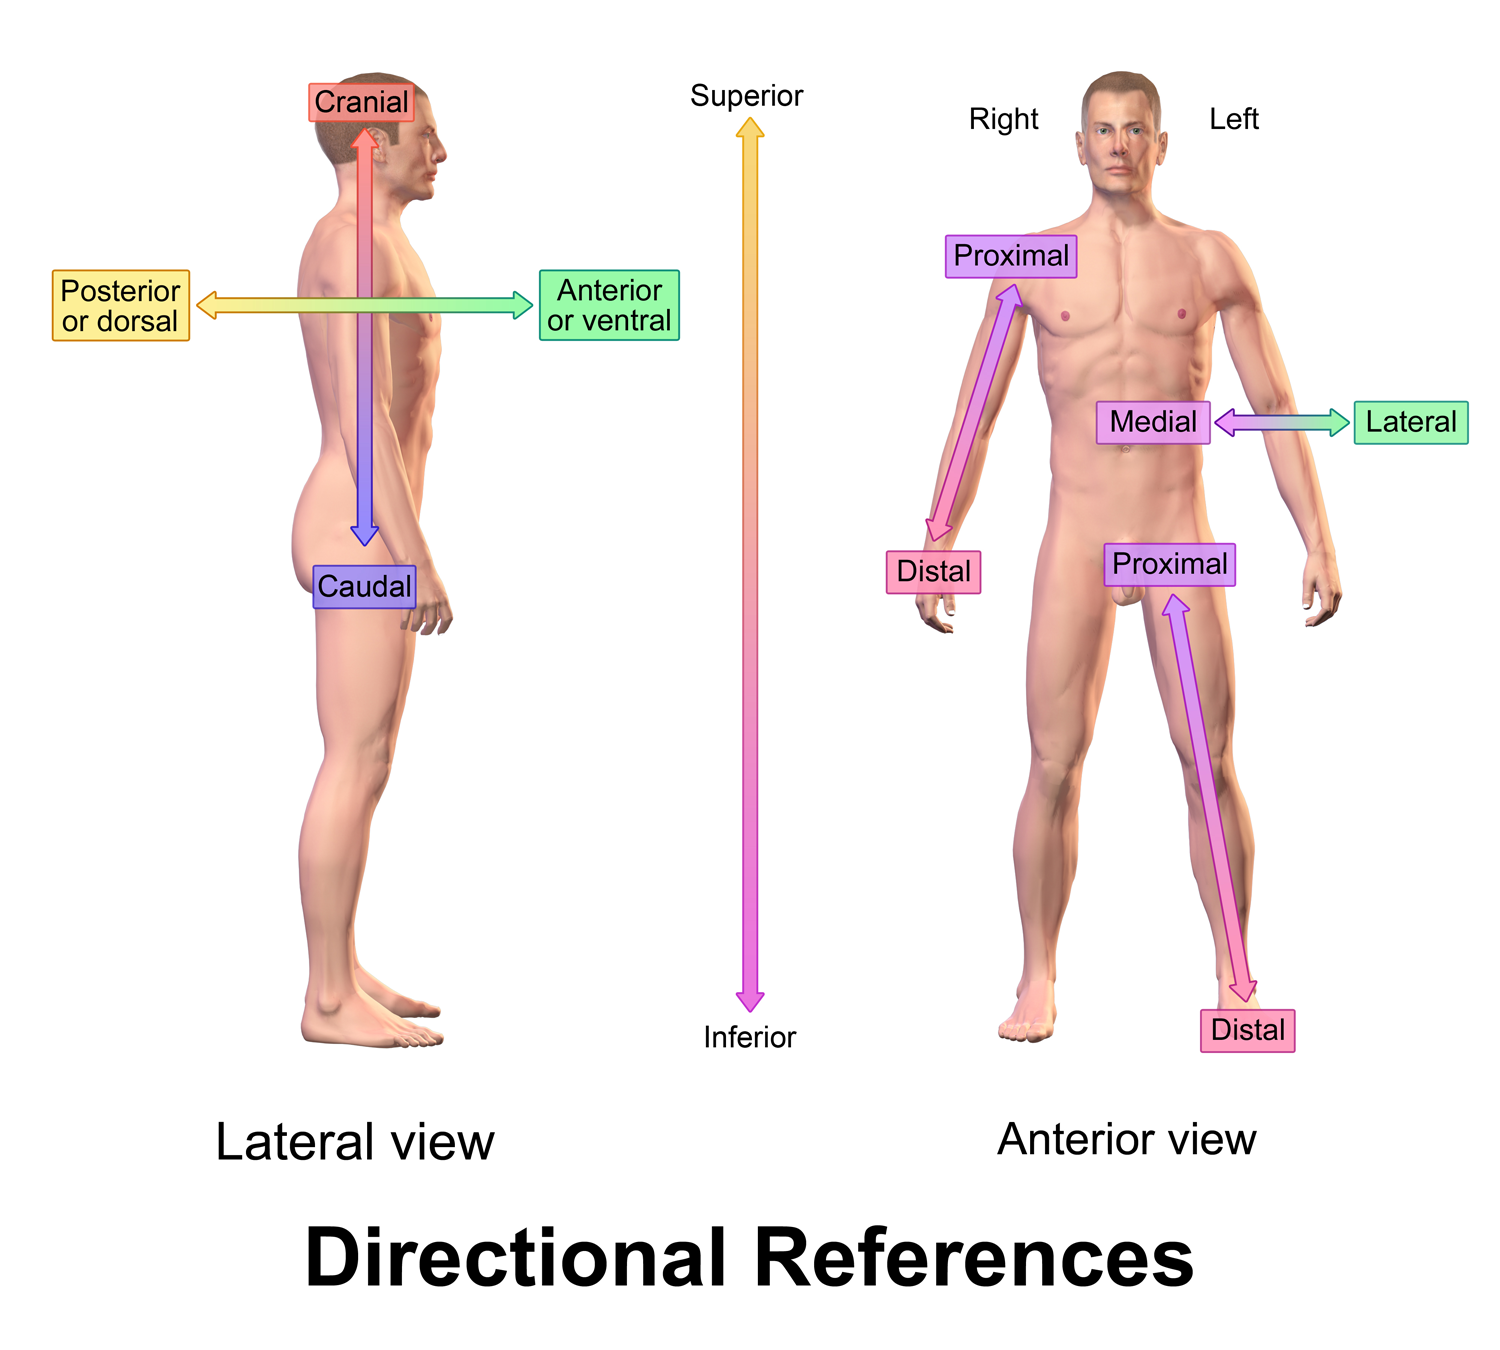
\includegraphics[width=0.9\linewidth]{img/Blausen_0019_AnatomicalDirectionalReferences.png}
  \caption{Anatomical directions}
  \label{fig:directions}
\end{figure}

\begin{table}[htbp]
  \centering
  \begin{tabularx}{\linewidth}{lX}
    \toprule
    Plane & Meaning \\
    \midrule
    midsagittal & plane that divides body into symmetrical halves \\
    sagittal & parallel to midsagittal, but divides into asymmetrical halves \\
    frontal/coronal & perpendicular to midsagittal, divides into anterior and posterior parts \\
    transverse & perpendicular to midsagittal, divides into superior and interior parts \\
    \bottomrule
  \end{tabularx}
  \caption{Anatomical planes}
  \label{tab:anatomical-planes}
\end{table}

\begin{figure}[htbp]
  \centering
  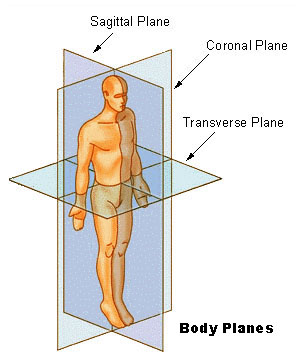
\includegraphics[width=0.6\linewidth]{img/BodyPlanes.jpg}
  \caption{Anatomical planes}
  \label{fig:planes}
\end{figure}

\paragraph{The main anatomical regions} are the \emph{axial} (head, neck, thorax, abdomen, pelvis) and \emph{appendicular} (upper and lower extremities) parts of the body.

\paragraph{The anatomical cavities} are
\begin{itemize}
  \item the dorsal cavity, which includes of the cranial and spinal cavity,
  \item the ventral cavity, which contains the thoracic and abdominopelvic cavities, separated by the diaphragm, and
  \item the smaller cavities (nasal, oral, orbital, tympanic, synovial).
\end{itemize}

\subsection{Cells}
Eukaryotic cells---cells in plants and animals---consist of a membrane, cytoplasm, DNA, and various organelles. They synthesize carbohydrates, lipids and proteins, all of which provide structure to the cells. The carbohydrates also transport/store energy. The lipids store (more) energy. There are many proteins. Enzymes catalyze reactions, others act as channels through membranes, signal activities, and defend against harmful bacteria. These are made from amino acids.

\subsubsection{Plasma membrane}
The plasma membrane surrounds the cell, and separates it from the environment. It is a two-layer shell of lipids with hydrophobic ends inward and -philic ends outward. Cholesterol is scattered in the membrane to stabilize it structurally. Protein channels in the membrane control the motion of substances in/out of the cell. Some substances can cross the membrane easily, while others must pass through protein channels. Osmosis is when substances are selectively passed through, and diffusion is when concentrations equalize across it. Osmosis requires energy in the form of ATP.

A typical cell has internal \chem{Na^+}

\subsubsection{Cytoplasm and organelles}
Cytoplasm is a fluid containing organellese, which are specialized ``small organs''. The nucleus contains DNA in the form of chromatin, inside of a membrane. Ribosomes are made in the nucleolus, inside the nucleus. Ribosomes leave the nucleus to synthesize proteins.

\subsection{Tissues}
\begin{itemize}
  \item Epitular tissue: Covers most surfaces, such as of skin and organs.
  \item Muscle tissue: Muscles, can be skeletal (attached to skeleton), smooth (in wall of blood vessels), or cardiac (only in the heart).
  \item Connective tissue: Holds everything together, several variations depending on what to hold together, including bone, fat, tendons, etc.
  \item Neural tissue: Neurons and glial cells that maintain the neurons.
\end{itemize}

\subsection{Organ systems}
11 systems, nervous and muscular most important:
\begin{itemize}
  \item Circulatory: The heart, blood, and veins. Moves nutrients and waste around, and regulates body temperature. The heart is made out of two pumps, consisting of two chambers each (one receives, one expels blood). Right pump sends blood to the lungs, left sends blood to the body. Two types of arteries, pulmonary (to/from lungs) and systemic (to/from body). A heartbeat begins with a pulse from pacemaker cells. This causes ions to move into the cells. This leads to the mechanical beating of the heart. In an electrocardiogram you can see de/polarization of atriums and ventriculars.
  \item Integumentary: Skin, hair, nails.
  \item Endocrine: Glands that secrete hormones.
  \item Lymphatic: Houses white blood cells, used as part of the immune system.
  \item Digestive: Mouth, esophagus, liver, stomach, small intestine, large intestine, rectum, anus.
  \item Urinary.
  \item Reproductive.
  \item Respiratory: Moves air to surfaces where diffusion between air and blood may happen. The conduction zone heats/humidifies/cleans incoming air. The respiratory zone (lungs) exchanges oxygen/co2 with the body. Properties of the lungs: Compliance (how easily they expand), elasticity (how easily they return to original size), surface tension (resistance to expansion). Volumes of the lungs: Tidal (air in/out of lungs during normal breathing), total capacity (maximum amount of air to breathe in), vital capacity (maximum breath out), residual (amount left when you have breathed out as much as possible).
  \item Skeletal: Protects, supports body, helps with motion, produces blood cells and stores minerals. A living system, cont being replaced.
    three types of joinery: fibrous (solid, immovable), brusk (allows some motion during compression or twist), sinovial (fluid-filled cavities, regular joints)
  \item Nervous: integrates and controls all bodily functions. central nervous system (encapsulated in bone, brain and spine), peripheral (everything else). can be divided also as somatic (non-autonomous control) and autonomous (everything that is done without consiocsness). latter divided into sympathic (fight or flight) and parasympathic (relaxing to normal condition when no danger). nervous system consists of neurons (cell body, axon, dendrites). dendrites receive signals, send them to axons. many neural circuits exist, such at convergent/divergent circuits. brain is the largest part of the nerv system: built off cerebrum (the two halves). frontal lobe (conscious action), isselapper (hud/muskelstimuli), tinningslapper, bakhodelappene.
    diencephalon: connect stem to halves. consists of thalamus, hypothalamus, apithalamus
    brainstem and small brain. stem connects brain to spine. small brain second largest part of brain, coordinates balance/position/timing and precision of movements
  \item Muscular: agonist (biceps), antagonist (triceps), synergist (assisting agonists).
    three types of tissue: cardiac (heart only). skeletal (connected to bone, skin, tendons). smooth muscle (surrounds tissue in most organs)
    slow and quick tissue, muscles consist of a mix of both.
    properties of muscle tissue: contractability, excitability, extensibility, elasticity (return to original shape).
\end{itemize}

\subsection{Homeostasis}
homeostasis: all systems of the body work to maintain a constant environment. homeostasis is the process where physical and chemical stuff is maintained in the face of external effects
extracellular fluid is important for this: surrounds cells, etc.
